% Options for packages loaded elsewhere
\PassOptionsToPackage{unicode}{hyperref}
\PassOptionsToPackage{hyphens}{url}
\PassOptionsToPackage{dvipsnames,svgnames,x11names}{xcolor}
%
\documentclass[
  letterpaper,
  DIV=11,
  numbers=noendperiod]{scrartcl}

\usepackage{amsmath,amssymb}
\usepackage{iftex}
\ifPDFTeX
  \usepackage[T1]{fontenc}
  \usepackage[utf8]{inputenc}
  \usepackage{textcomp} % provide euro and other symbols
\else % if luatex or xetex
  \usepackage{unicode-math}
  \defaultfontfeatures{Scale=MatchLowercase}
  \defaultfontfeatures[\rmfamily]{Ligatures=TeX,Scale=1}
\fi
\usepackage{lmodern}
\ifPDFTeX\else  
    % xetex/luatex font selection
\fi
% Use upquote if available, for straight quotes in verbatim environments
\IfFileExists{upquote.sty}{\usepackage{upquote}}{}
\IfFileExists{microtype.sty}{% use microtype if available
  \usepackage[]{microtype}
  \UseMicrotypeSet[protrusion]{basicmath} % disable protrusion for tt fonts
}{}
\makeatletter
\@ifundefined{KOMAClassName}{% if non-KOMA class
  \IfFileExists{parskip.sty}{%
    \usepackage{parskip}
  }{% else
    \setlength{\parindent}{0pt}
    \setlength{\parskip}{6pt plus 2pt minus 1pt}}
}{% if KOMA class
  \KOMAoptions{parskip=half}}
\makeatother
\usepackage{xcolor}
\setlength{\emergencystretch}{3em} % prevent overfull lines
\setcounter{secnumdepth}{-\maxdimen} % remove section numbering
% Make \paragraph and \subparagraph free-standing
\makeatletter
\ifx\paragraph\undefined\else
  \let\oldparagraph\paragraph
  \renewcommand{\paragraph}{
    \@ifstar
      \xxxParagraphStar
      \xxxParagraphNoStar
  }
  \newcommand{\xxxParagraphStar}[1]{\oldparagraph*{#1}\mbox{}}
  \newcommand{\xxxParagraphNoStar}[1]{\oldparagraph{#1}\mbox{}}
\fi
\ifx\subparagraph\undefined\else
  \let\oldsubparagraph\subparagraph
  \renewcommand{\subparagraph}{
    \@ifstar
      \xxxSubParagraphStar
      \xxxSubParagraphNoStar
  }
  \newcommand{\xxxSubParagraphStar}[1]{\oldsubparagraph*{#1}\mbox{}}
  \newcommand{\xxxSubParagraphNoStar}[1]{\oldsubparagraph{#1}\mbox{}}
\fi
\makeatother

\usepackage{color}
\usepackage{fancyvrb}
\newcommand{\VerbBar}{|}
\newcommand{\VERB}{\Verb[commandchars=\\\{\}]}
\DefineVerbatimEnvironment{Highlighting}{Verbatim}{commandchars=\\\{\}}
% Add ',fontsize=\small' for more characters per line
\usepackage{framed}
\definecolor{shadecolor}{RGB}{241,243,245}
\newenvironment{Shaded}{\begin{snugshade}}{\end{snugshade}}
\newcommand{\AlertTok}[1]{\textcolor[rgb]{0.68,0.00,0.00}{#1}}
\newcommand{\AnnotationTok}[1]{\textcolor[rgb]{0.37,0.37,0.37}{#1}}
\newcommand{\AttributeTok}[1]{\textcolor[rgb]{0.40,0.45,0.13}{#1}}
\newcommand{\BaseNTok}[1]{\textcolor[rgb]{0.68,0.00,0.00}{#1}}
\newcommand{\BuiltInTok}[1]{\textcolor[rgb]{0.00,0.23,0.31}{#1}}
\newcommand{\CharTok}[1]{\textcolor[rgb]{0.13,0.47,0.30}{#1}}
\newcommand{\CommentTok}[1]{\textcolor[rgb]{0.37,0.37,0.37}{#1}}
\newcommand{\CommentVarTok}[1]{\textcolor[rgb]{0.37,0.37,0.37}{\textit{#1}}}
\newcommand{\ConstantTok}[1]{\textcolor[rgb]{0.56,0.35,0.01}{#1}}
\newcommand{\ControlFlowTok}[1]{\textcolor[rgb]{0.00,0.23,0.31}{\textbf{#1}}}
\newcommand{\DataTypeTok}[1]{\textcolor[rgb]{0.68,0.00,0.00}{#1}}
\newcommand{\DecValTok}[1]{\textcolor[rgb]{0.68,0.00,0.00}{#1}}
\newcommand{\DocumentationTok}[1]{\textcolor[rgb]{0.37,0.37,0.37}{\textit{#1}}}
\newcommand{\ErrorTok}[1]{\textcolor[rgb]{0.68,0.00,0.00}{#1}}
\newcommand{\ExtensionTok}[1]{\textcolor[rgb]{0.00,0.23,0.31}{#1}}
\newcommand{\FloatTok}[1]{\textcolor[rgb]{0.68,0.00,0.00}{#1}}
\newcommand{\FunctionTok}[1]{\textcolor[rgb]{0.28,0.35,0.67}{#1}}
\newcommand{\ImportTok}[1]{\textcolor[rgb]{0.00,0.46,0.62}{#1}}
\newcommand{\InformationTok}[1]{\textcolor[rgb]{0.37,0.37,0.37}{#1}}
\newcommand{\KeywordTok}[1]{\textcolor[rgb]{0.00,0.23,0.31}{\textbf{#1}}}
\newcommand{\NormalTok}[1]{\textcolor[rgb]{0.00,0.23,0.31}{#1}}
\newcommand{\OperatorTok}[1]{\textcolor[rgb]{0.37,0.37,0.37}{#1}}
\newcommand{\OtherTok}[1]{\textcolor[rgb]{0.00,0.23,0.31}{#1}}
\newcommand{\PreprocessorTok}[1]{\textcolor[rgb]{0.68,0.00,0.00}{#1}}
\newcommand{\RegionMarkerTok}[1]{\textcolor[rgb]{0.00,0.23,0.31}{#1}}
\newcommand{\SpecialCharTok}[1]{\textcolor[rgb]{0.37,0.37,0.37}{#1}}
\newcommand{\SpecialStringTok}[1]{\textcolor[rgb]{0.13,0.47,0.30}{#1}}
\newcommand{\StringTok}[1]{\textcolor[rgb]{0.13,0.47,0.30}{#1}}
\newcommand{\VariableTok}[1]{\textcolor[rgb]{0.07,0.07,0.07}{#1}}
\newcommand{\VerbatimStringTok}[1]{\textcolor[rgb]{0.13,0.47,0.30}{#1}}
\newcommand{\WarningTok}[1]{\textcolor[rgb]{0.37,0.37,0.37}{\textit{#1}}}

\providecommand{\tightlist}{%
  \setlength{\itemsep}{0pt}\setlength{\parskip}{0pt}}\usepackage{longtable,booktabs,array}
\usepackage{calc} % for calculating minipage widths
% Correct order of tables after \paragraph or \subparagraph
\usepackage{etoolbox}
\makeatletter
\patchcmd\longtable{\par}{\if@noskipsec\mbox{}\fi\par}{}{}
\makeatother
% Allow footnotes in longtable head/foot
\IfFileExists{footnotehyper.sty}{\usepackage{footnotehyper}}{\usepackage{footnote}}
\makesavenoteenv{longtable}
\usepackage{graphicx}
\makeatletter
\def\maxwidth{\ifdim\Gin@nat@width>\linewidth\linewidth\else\Gin@nat@width\fi}
\def\maxheight{\ifdim\Gin@nat@height>\textheight\textheight\else\Gin@nat@height\fi}
\makeatother
% Scale images if necessary, so that they will not overflow the page
% margins by default, and it is still possible to overwrite the defaults
% using explicit options in \includegraphics[width, height, ...]{}
\setkeys{Gin}{width=\maxwidth,height=\maxheight,keepaspectratio}
% Set default figure placement to htbp
\makeatletter
\def\fps@figure{htbp}
\makeatother

\usepackage{float}
\usepackage{tabularray}
\usepackage[normalem]{ulem}
\usepackage{graphicx}
\UseTblrLibrary{booktabs}
\UseTblrLibrary{rotating}
\UseTblrLibrary{siunitx}
\NewTableCommand{\tinytableDefineColor}[3]{\definecolor{#1}{#2}{#3}}
\newcommand{\tinytableTabularrayUnderline}[1]{\underline{#1}}
\newcommand{\tinytableTabularrayStrikeout}[1]{\sout{#1}}
\KOMAoption{captions}{tableheading}
\makeatletter
\@ifpackageloaded{caption}{}{\usepackage{caption}}
\AtBeginDocument{%
\ifdefined\contentsname
  \renewcommand*\contentsname{Table of contents}
\else
  \newcommand\contentsname{Table of contents}
\fi
\ifdefined\listfigurename
  \renewcommand*\listfigurename{List of Figures}
\else
  \newcommand\listfigurename{List of Figures}
\fi
\ifdefined\listtablename
  \renewcommand*\listtablename{List of Tables}
\else
  \newcommand\listtablename{List of Tables}
\fi
\ifdefined\figurename
  \renewcommand*\figurename{Figure}
\else
  \newcommand\figurename{Figure}
\fi
\ifdefined\tablename
  \renewcommand*\tablename{Table}
\else
  \newcommand\tablename{Table}
\fi
}
\@ifpackageloaded{float}{}{\usepackage{float}}
\floatstyle{ruled}
\@ifundefined{c@chapter}{\newfloat{codelisting}{h}{lop}}{\newfloat{codelisting}{h}{lop}[chapter]}
\floatname{codelisting}{Listing}
\newcommand*\listoflistings{\listof{codelisting}{List of Listings}}
\makeatother
\makeatletter
\makeatother
\makeatletter
\@ifpackageloaded{caption}{}{\usepackage{caption}}
\@ifpackageloaded{subcaption}{}{\usepackage{subcaption}}
\makeatother

\ifLuaTeX
  \usepackage{selnolig}  % disable illegal ligatures
\fi
\usepackage{bookmark}

\IfFileExists{xurl.sty}{\usepackage{xurl}}{} % add URL line breaks if available
\urlstyle{same} % disable monospaced font for URLs
\hypersetup{
  pdftitle={Simulated Grant Data},
  colorlinks=true,
  linkcolor={blue},
  filecolor={Maroon},
  citecolor={Blue},
  urlcolor={Blue},
  pdfcreator={LaTeX via pandoc}}


\title{Simulated Grant Data}
\author{}
\date{}

\begin{document}
\maketitle


\subsection{Overview}\label{overview}

The code below attempts to create a simulated dataset for the purposes
of evaluating how factors such as the level of expertise (high, medium,
low, not enough) and role (reviewer, panelist) might impact overall
scores.

The unit of observation is the application and basic structure attempts
to mimic the multilevel nature of the review process for the CIHR
Project Grant competitions. There are roughly 50 CIHR Committees, and
each committee has around 25 or so members. In practice the number of
total applications may vary quite a lot across committees (e.g., up to
50 for PH1 or PH2 when I was SO); however since we are focused on the
evaluation of overall scores \emph{among those proposals discussed}
(i.e., excluding those streamlined), this is likely closer to 15 or so
proposals per committee (again, my reference is PH committees).

In the code below we specify 50 committees, 15 discussed applications
per committee, and 24 members per committee.

The code below is annotated with some simple coefficients for reviewer
status and expertise (no interaction).

First, load the packages needed for this setup and analysis

\begin{Shaded}
\begin{Highlighting}[]
\CommentTok{\# list of packages needed}
\NormalTok{pkgs }\OtherTok{\textless{}{-}} \FunctionTok{c}\NormalTok{(}\StringTok{\textquotesingle{}here\textquotesingle{}}\NormalTok{, }\StringTok{\textquotesingle{}tidyverse\textquotesingle{}}\NormalTok{, }\StringTok{\textquotesingle{}faux\textquotesingle{}}\NormalTok{, }\StringTok{\textquotesingle{}modelsummary\textquotesingle{}}\NormalTok{, }
  \StringTok{\textquotesingle{}fixest\textquotesingle{}}\NormalTok{, }\StringTok{\textquotesingle{}tinytable\textquotesingle{}}\NormalTok{, }\StringTok{\textquotesingle{}marginaleffects\textquotesingle{}}\NormalTok{,}
  \StringTok{\textquotesingle{}truncnorm\textquotesingle{}}\NormalTok{, }\StringTok{\textquotesingle{}lme4\textquotesingle{}}\NormalTok{)}

\CommentTok{\# install any needed packages}
\CommentTok{\# install.packages(pkgs)}

\CommentTok{\# load all packages at once}
\FunctionTok{lapply}\NormalTok{(pkgs, library, }\AttributeTok{character.only=}\ConstantTok{TRUE}\NormalTok{)}
\end{Highlighting}
\end{Shaded}

Now we set up the basic parameters and multilevel structure for the
simulated data. Note that since we are focused on those applications
that are not streamlined and make it to discussion, the distribution of
the overall score is truncated. CIHR places an upper limit of 4.9 for
the highest ranking and in many cases a lower level of 3.5 is used
(though not the only criteria) to draw the line below which applications
are streamlined.

\begin{Shaded}
\begin{Highlighting}[]
\CommentTok{\# set seed for reproducibility}
\FunctionTok{set.seed}\NormalTok{(}\DecValTok{4875}\NormalTok{)}

\CommentTok{\# define parameters}
\NormalTok{cmte\_n }\OtherTok{=} \DecValTok{50}      \CommentTok{\# number of committees}
\NormalTok{app\_n }\OtherTok{=} \DecValTok{15}       \CommentTok{\# number of discussed applications}
\NormalTok{mem\_n }\OtherTok{=} \DecValTok{24}       \CommentTok{\# number of committee members}
\NormalTok{b0 }\OtherTok{=} \FloatTok{4.1}         \CommentTok{\# intercept for average score}
\NormalTok{b1 }\OtherTok{=} \FloatTok{0.2}         \CommentTok{\# fixed effect of panelist vs. reviewer }
\NormalTok{b2 }\OtherTok{=} \SpecialCharTok{{-}}\FloatTok{0.1}        \CommentTok{\# fixed effect of high expertise}
\NormalTok{b3 }\OtherTok{=} \FloatTok{0.1}         \CommentTok{\# fixed effect of low expertise}
\NormalTok{b4 }\OtherTok{=} \FloatTok{0.2}         \CommentTok{\# fixed effect of no expertise}
\NormalTok{u0c\_sd }\OtherTok{=} \FloatTok{0.1}     \CommentTok{\# random intercept SD for committee}
\NormalTok{u0m\_sd }\OtherTok{=} \FloatTok{0.2}     \CommentTok{\# random intercept SD for members}
\NormalTok{u0a\_sd }\OtherTok{=} \FloatTok{0.2}     \CommentTok{\# random intercept SD for applications}
\NormalTok{sigma\_sd }\OtherTok{=} \FloatTok{0.2}   \CommentTok{\# error SD for overall scores}
\NormalTok{score\_min }\OtherTok{=} \FloatTok{3.5}  \CommentTok{\# lower bound for score}
\NormalTok{score\_max }\OtherTok{=} \FloatTok{4.9}  \CommentTok{\# upper bound for score}

\CommentTok{\# set up data structure}
\NormalTok{data }\OtherTok{\textless{}{-}} \FunctionTok{add\_random}\NormalTok{(}\AttributeTok{committee =}\NormalTok{ cmte\_n, }
  \AttributeTok{application =}\NormalTok{ app\_n, }\AttributeTok{member =}\NormalTok{ mem\_n) }\SpecialCharTok{|\textgreater{}}
  
  \CommentTok{\# recode values for committee, application, and member}
  \FunctionTok{add\_between}\NormalTok{(}\StringTok{"committee"}\NormalTok{, }
    \AttributeTok{cmte =} \FunctionTok{sprintf}\NormalTok{(}\StringTok{"\%02d"}\NormalTok{, }\DecValTok{1}\SpecialCharTok{:}\NormalTok{cmte\_n)) }\SpecialCharTok{|\textgreater{}}
  \FunctionTok{add\_between}\NormalTok{(}\StringTok{"application"}\NormalTok{,}
    \AttributeTok{app =} \DecValTok{1}\SpecialCharTok{:}\NormalTok{app\_n) }\SpecialCharTok{|\textgreater{}}
  \FunctionTok{add\_between}\NormalTok{(}\StringTok{"member"}\NormalTok{, }
    \AttributeTok{memno =} \FunctionTok{sprintf}\NormalTok{(}\StringTok{"\%02d"}\NormalTok{, }\DecValTok{1}\SpecialCharTok{:}\NormalTok{mem\_n)) }\SpecialCharTok{|\textgreater{}}
  
  \CommentTok{\# create unique ID for each committee member}
  \FunctionTok{mutate}\NormalTok{(}\AttributeTok{cid =} \FunctionTok{paste0}\NormalTok{(cmte, }\StringTok{"\_"}\NormalTok{, memno)) }\SpecialCharTok{|\textgreater{}}
 
  \CommentTok{\# assign reviewers uniquely within each application}
  \FunctionTok{group\_by}\NormalTok{(cmte, app) }\SpecialCharTok{|\textgreater{}}
  \FunctionTok{mutate}\NormalTok{(}
    \AttributeTok{job =} \FunctionTok{sample}\NormalTok{(}\FunctionTok{c}\NormalTok{(}\FunctionTok{rep}\NormalTok{(}\StringTok{"reviewer"}\NormalTok{, }\DecValTok{3}\NormalTok{), }
      \FunctionTok{rep}\NormalTok{(}\StringTok{"panelist"}\NormalTok{, }\DecValTok{21}\NormalTok{))),}
    \CommentTok{\# add expertise for each member}
    \AttributeTok{exp =} \FunctionTok{sample}\NormalTok{(}\FunctionTok{c}\NormalTok{(}\FunctionTok{rep}\NormalTok{(}\StringTok{"high"}\NormalTok{, }\DecValTok{6}\NormalTok{), }
      \FunctionTok{rep}\NormalTok{(}\StringTok{"med"}\NormalTok{, }\DecValTok{10}\NormalTok{), }\FunctionTok{rep}\NormalTok{(}\StringTok{"low"}\NormalTok{, }\DecValTok{4}\NormalTok{),}
      \FunctionTok{rep}\NormalTok{(}\StringTok{"none"}\NormalTok{, }\DecValTok{4}\NormalTok{)))) }\SpecialCharTok{|\textgreater{}}
  \FunctionTok{ungroup}\NormalTok{() }\SpecialCharTok{|\textgreater{}}
  
  \CommentTok{\# add indicators for reviewer, expertise}
  \FunctionTok{mutate}\NormalTok{(}
    \AttributeTok{panelist =} \FunctionTok{if\_else}\NormalTok{(job }\SpecialCharTok{==} \StringTok{"panelist"}\NormalTok{, }\DecValTok{1}\NormalTok{, }\DecValTok{0}\NormalTok{),}
    \AttributeTok{exp\_high =} \FunctionTok{if\_else}\NormalTok{(exp }\SpecialCharTok{==} \StringTok{"high"}\NormalTok{, }\DecValTok{1}\NormalTok{, }\DecValTok{0}\NormalTok{),}
    \AttributeTok{exp\_low =} \FunctionTok{if\_else}\NormalTok{(exp }\SpecialCharTok{==} \StringTok{"low"}\NormalTok{, }\DecValTok{1}\NormalTok{, }\DecValTok{0}\NormalTok{),}
    \AttributeTok{exp\_none =} \FunctionTok{if\_else}\NormalTok{(exp }\SpecialCharTok{==} \StringTok{"none"}\NormalTok{, }\DecValTok{1}\NormalTok{, }\DecValTok{0}\NormalTok{)}
\NormalTok{  ) }\SpecialCharTok{|\textgreater{}}
  
  \CommentTok{\# add random effects }
  \FunctionTok{add\_ranef}\NormalTok{(}\StringTok{"cmte"}\NormalTok{, }\AttributeTok{u0c =}\NormalTok{ u0c\_sd) }\SpecialCharTok{|\textgreater{}}
  \FunctionTok{add\_ranef}\NormalTok{(}\StringTok{"member"}\NormalTok{, }\AttributeTok{u0m =}\NormalTok{ u0m\_sd) }\SpecialCharTok{|\textgreater{}}
  \FunctionTok{add\_ranef}\NormalTok{(}\StringTok{"application"}\NormalTok{, }\AttributeTok{u0a =}\NormalTok{ u0a\_sd) }\SpecialCharTok{|\textgreater{}}
  \FunctionTok{add\_ranef}\NormalTok{(}\AttributeTok{sigma =}\NormalTok{ sigma\_sd) }\SpecialCharTok{|\textgreater{}}

  \CommentTok{\# Compute score using a truncated normal distribution}
  \FunctionTok{mutate}\NormalTok{(}
    \AttributeTok{score =} \FunctionTok{rtruncnorm}\NormalTok{(}\FunctionTok{n}\NormalTok{(), }\AttributeTok{a =}\NormalTok{ score\_min, }\AttributeTok{b =}\NormalTok{ score\_max, }
      \AttributeTok{mean =}\NormalTok{ b0 }\SpecialCharTok{+}\NormalTok{ u0c }\SpecialCharTok{+}\NormalTok{ u0m }\SpecialCharTok{+}\NormalTok{ u0a }\SpecialCharTok{+}
\NormalTok{        (b1 }\SpecialCharTok{*}\NormalTok{ panelist) }\SpecialCharTok{+}\NormalTok{ (b2 }\SpecialCharTok{*}\NormalTok{ exp\_high) }\SpecialCharTok{+}
\NormalTok{        (b3 }\SpecialCharTok{*}\NormalTok{ exp\_low) }\SpecialCharTok{+}\NormalTok{ (b4 }\SpecialCharTok{*}\NormalTok{ exp\_none), }
      \AttributeTok{sd =}\NormalTok{ sigma\_sd)}
\NormalTok{  ) }\SpecialCharTok{|\textgreater{}} 
  
  \CommentTok{\# drop intermediate variables}
  \FunctionTok{select}\NormalTok{(}\SpecialCharTok{{-}}\NormalTok{committee, }\SpecialCharTok{{-}}\NormalTok{application, }\SpecialCharTok{{-}}\NormalTok{member,}
         \SpecialCharTok{{-}}\NormalTok{u0c, }\SpecialCharTok{{-}}\NormalTok{u0m, }\SpecialCharTok{{-}}\NormalTok{u0a, }\SpecialCharTok{{-}}\NormalTok{sigma)}
\end{Highlighting}
\end{Shaded}

Here is a glimpse of the data structure:

\begin{Shaded}
\begin{Highlighting}[]
\FunctionTok{tt}\NormalTok{(}\FunctionTok{head}\NormalTok{(data))}
\end{Highlighting}
\end{Shaded}

\begin{table}
\centering
\begin{tblr}[         %% tabularray outer open
]                     %% tabularray outer close
{                     %% tabularray inner open
colspec={Q[]Q[]Q[]Q[]Q[]Q[]Q[]Q[]Q[]Q[]Q[]},
}                     %% tabularray inner close
\toprule
cmte & app & memno & cid & job & exp & panelist & exp_high & exp_low & exp_none & score \\ \midrule %% TinyTableHeader
01 & 1 & 01 & 01_01 & panelist & none & 1 & 0 & 0 & 1 & 4.426219 \\
01 & 1 & 02 & 01_02 & panelist & med  & 1 & 0 & 0 & 0 & 4.491622 \\
01 & 1 & 03 & 01_03 & panelist & med  & 1 & 0 & 0 & 0 & 3.926662 \\
01 & 1 & 04 & 01_04 & reviewer & none & 0 & 0 & 0 & 1 & 3.932127 \\
01 & 1 & 05 & 01_05 & panelist & high & 1 & 1 & 0 & 0 & 3.956093 \\
01 & 1 & 06 & 01_06 & panelist & low  & 1 & 0 & 1 & 0 & 4.350588 \\
\bottomrule
\end{tblr}
\end{table}

And a simple histogram of the distribution of overall scores:

\begin{Shaded}
\begin{Highlighting}[]
\FunctionTok{ggplot}\NormalTok{(data, }\FunctionTok{aes}\NormalTok{(}\AttributeTok{x =}\NormalTok{ score)) }\SpecialCharTok{+} \FunctionTok{geom\_histogram}\NormalTok{() }\SpecialCharTok{+}
         \FunctionTok{theme\_classic}\NormalTok{()}
\end{Highlighting}
\end{Shaded}

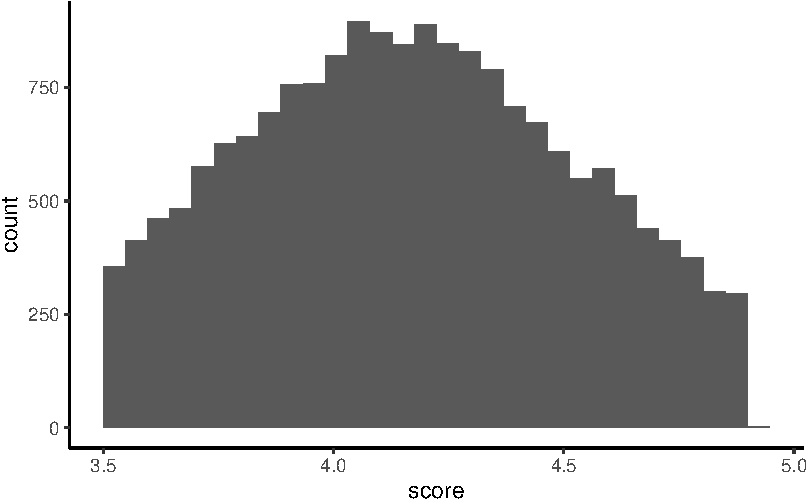
\includegraphics{sim-data_files/figure-pdf/unnamed-chunk-4-1.pdf}

A simple set of models with random effects for committee, member, and
application, and fixed effects for whether or not the score comes from a
panelist and various levels of expertise (should probably be estimated
by interval regression or some other way of accounting for the truncated
distribution of the outcome, but later):

\begin{Shaded}
\begin{Highlighting}[]
\CommentTok{\# empty}
\NormalTok{m0 }\OtherTok{\textless{}{-}} \FunctionTok{lmer}\NormalTok{(score }\SpecialCharTok{\textasciitilde{}} \DecValTok{1} \SpecialCharTok{+}\NormalTok{ (}\DecValTok{1} \SpecialCharTok{|}\NormalTok{ cmte) }\SpecialCharTok{+}\NormalTok{ (}\DecValTok{1} \SpecialCharTok{|}\NormalTok{ memno) }\SpecialCharTok{+}
\NormalTok{  (}\DecValTok{1} \SpecialCharTok{|}\NormalTok{ app), }\AttributeTok{data =}\NormalTok{ data)}

\CommentTok{\# add reviewer}
\NormalTok{m1 }\OtherTok{\textless{}{-}} \FunctionTok{lmer}\NormalTok{(score }\SpecialCharTok{\textasciitilde{}} \DecValTok{1} \SpecialCharTok{+}\NormalTok{ panelist }\SpecialCharTok{+}\NormalTok{ (}\DecValTok{1} \SpecialCharTok{|}\NormalTok{ cmte) }\SpecialCharTok{+} 
\NormalTok{  (}\DecValTok{1} \SpecialCharTok{|}\NormalTok{ memno) }\SpecialCharTok{+}\NormalTok{ (}\DecValTok{1} \SpecialCharTok{|}\NormalTok{ app), }\AttributeTok{data =}\NormalTok{ data)}

\CommentTok{\# add expertise}
\NormalTok{m2 }\OtherTok{\textless{}{-}} \FunctionTok{lmer}\NormalTok{(score }\SpecialCharTok{\textasciitilde{}} \DecValTok{1} \SpecialCharTok{+}\NormalTok{ panelist }\SpecialCharTok{+}\NormalTok{ exp\_high }\SpecialCharTok{+}\NormalTok{ exp\_low }\SpecialCharTok{+}
\NormalTok{  exp\_none }\SpecialCharTok{+}\NormalTok{ (}\DecValTok{1} \SpecialCharTok{|}\NormalTok{ cmte) }\SpecialCharTok{+}\NormalTok{ (}\DecValTok{1} \SpecialCharTok{|}\NormalTok{ memno) }\SpecialCharTok{+}\NormalTok{ (}\DecValTok{1} \SpecialCharTok{|}\NormalTok{ app), }
  \AttributeTok{data =}\NormalTok{ data)}

\FunctionTok{modelsummary}\NormalTok{(}\FunctionTok{list}\NormalTok{(}\StringTok{"Empty"} \OtherTok{=}\NormalTok{ m0, }
  \StringTok{"+ Reviewer"} \OtherTok{=}\NormalTok{ m1, }\StringTok{"+ Expertise"} \OtherTok{=}\NormalTok{ m2),}
  \AttributeTok{gof\_omit =} \StringTok{\textquotesingle{}DF|Deviance|R2|AIC|BIC|RMSE\textquotesingle{}}\NormalTok{,}
  \AttributeTok{escape =} \ConstantTok{TRUE}\NormalTok{)}
\end{Highlighting}
\end{Shaded}

\begin{table}
\centering
\begin{tblr}[         %% tabularray outer open
]                     %% tabularray outer close
{                     %% tabularray inner open
colspec={Q[]Q[]Q[]Q[]},
column{1}={halign=l,},
column{2}={halign=c,},
column{3}={halign=c,},
column{4}={halign=c,},
hline{16}={1,2,3,4}{solid, 0.05em, black},
}                     %% tabularray inner close
\toprule
& Empty & + Reviewer & + Expertise \\ \midrule %% TinyTableHeader
(Intercept)          & \num{4.172}   & \num{4.023}   & \num{4.001}   \\
& (\num{0.064}) & (\num{0.064}) & (\num{0.064}) \\
panelist             &                & \num{0.171}   & \num{0.170}   \\
&                & (\num{0.005}) & (\num{0.004}) \\
exp\_high           &                &                & \num{-0.083}  \\
&                &                & (\num{0.004}) \\
exp\_low            &                &                & \num{0.088}   \\
&                &                & (\num{0.004}) \\
exp\_none           &                &                & \num{0.176}   \\
&                &                & (\num{0.004}) \\
SD (Intercept cmte)  & \num{0.078}   & \num{0.078}   & \num{0.078}   \\
SD (Intercept memno) & \num{0.190}   & \num{0.189}   & \num{0.188}   \\
SD (Intercept app)   & \num{0.191}   & \num{0.191}   & \num{0.191}   \\
SD (Observations)    & \num{0.216}   & \num{0.208}   & \num{0.189}   \\
Num.Obs.             & \num{18000}   & \num{18000}   & \num{18000}   \\
ICC                  & \num{0.6}     & \num{0.6}     & \num{0.7}     \\
\bottomrule
\end{tblr}
\end{table}




\end{document}
